% HW1 for Intro to Data Science
% also my first real foray into LaTeX ._.

\documentclass{article} 
\usepackage{fancyhdr, titling, graphicx, mathtools, fixltx2e, tikz, lastpage}
\pagestyle{fancy}
\usetikzlibrary{positioning}
\newdimen\nodeDist
\nodeDist=35mm

\fancyhead[L]{Green, Ben}
\fancyhead[R]{Page \thepage\ of \pageref{LastPage}}
\fancyfoot{}

\author{Ben Green}
\title{Intro to Data Science HW 3}

\begin{document}

% title page
\begin{titlepage}
	\begin{center}
	\textsc{\LARGE Intro to Data Science HW 3}\\
	\vspace{3mm}
	
	{\large \theauthor}\\
	
	\tableofcontents
	\setcounter{secnumdepth}{0}
	\vfill
	
	{\large \today}
	\end{center}

\end{titlepage}

\section{Question 1}

\begin{center}
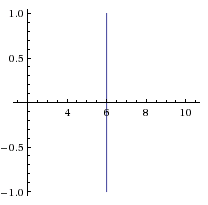
\includegraphics{q1.png}
\end{center}

where x1 is the horizontal axis, x2 is the vertical axis, objects to the right of the line are + and objects to the left are -.

\section{Question 2}
x - 14x4\\
$\theta$ - 4x1\\
y - 4x1

\section{Question 3}

\subsection{3a}
Feature scaling is necessary because the classifier (midterm exam)$^2$'s range of data value varies widely. One strategy that we can use is rescaling.

\subsection{3b}
Decrease the learning rate until we have $j\theta$ decrease over time.

\section{Question 4}

\subsection{4a}
Boosting can fail to perform well given overly complex base classifiers or base classifiers that are too weak.

\subsection{4b}
Boosting weak base classifiers (or vice versa if necessary) can provide a significant improvement in performance. Brownboosting also deemphasizes outliers which may help.

\section{Question 5}

\subsection{5a}
The SVM is making an underfit which means the classifier has high bias and low variance. 

\subsection{5b}
C should be increased.

\subsection{5c}
$\sigma^2$ should be decreased.

\section{Question 6}

Bagging can reduce predictive accuracy and is computationally hard.

\section{Question 7}
Na{\"i}ve Bayesian classification is called na{\"i}ve because it assumes class conditional independence. That is, the effect of an attribute value on a given class is independent of
the values of the other attributes. This assumption is made to reduce computational costs, and hence is considered na{\"i}ve.

\section{Question 8}
Accuracy - 95/1000 = .095\\
Recall - 85/100 = .85\\
Precision - 85/975 = .087\\
F1-score - 2*product/sum of precision \& recall = .158

\section{Question 9}

\subsection{9a}
The accuracy would be .99. This would be a bad fraud detection system because fraud is not actually ever being detected.

\subsection{9b}

Recall - 1\\
Precision - .01

\section{Question 10}
Led7 is the specified point.\\

\noindent The Z-statistic is .16.

\section {Question 11}

\subsection{11a}
Minimize the Schwarz criterion.

\subsection{11b}
This results in a low amount of distortion


\section{Question 12}
Spectral clustering is optimal because it isn't NP complete.

\section{Question 13}

\subsection{13a}
The SSE for cluster C1 is 36.

\subsection{13b}
The optimal partitioning splits C1 into two groups - one with (0,8) and one with (6,5) and (3,2)

\subsection{13c}
The new SSE is 9, so the reduction is 27.

\section{Question 14}
Point 3 fits these criteria.

\section{Question 15}
B, C, F, B






\end{document}